\documentclass[10pt,letterpaper]{article}

\usepackage{hyperref}
\usepackage{cogsci}
\usepackage{pslatex}
\usepackage{apacite}
\usepackage{graphicx}
\usepackage{todonotes}
\usepackage{caption}
\usepackage{subcaption}

\title{Extremely costly intensifiers are stronger than quite costly ones.}
 
\author{{\large \bf Erin Bennett (erindb@stanford.edu)} \\
  Department of Psychology, 450 Serra Mall , Stanford, CA 94305
  \AND {\large \bf Noah Goodman (ngoodman@stanford.edu)} \\
  Department of Psychology, 450 Serra Mall , Stanford, CA 94305}


\begin{document}

\maketitle


\begin{abstract}
%Intensifiers of scalar adjectives might derive the degree of their meaning from their cost.
%We show that surprisal and syllable length, two different construals of the cost of an intensifier, both independently predict estimates of degree.
%We further show that when an intensifier is frequently repeated within a ``non-standard dialect of English'' (i.e. when we manipulate the surprisal of an intensifier), its inferred degree is consequently lower.

\todo[inline]{abstract}

\textbf{Keywords:} 
intensifiers; degree adverbs; scalar adjectives; pragmatics; m-implicature
\end{abstract}


\section{Introduction}

\todo[inline]{i need to clean this up}

%form / meaning / and meaning-setting information -- distinguish the three in discussion.

%for the intro, i think we will want to explore a bit the question of arbitrariness of word meaning: http://en.wikipedia.org/wiki/Sign_(linguistics) . it's good to start with and example and with a big picture question. so it might be something like: why is an "extremely good paper" better than a "quite good paper"? the traditional answer is that these words simply have different meanings which have been arbitrarily and conventionally assigned to their forms. in this paper we explore the hypothesis that the meanings of intensifiers are at least partly non-arbitrary, but instead are determined by aspects of their production (or comprehension) cost. then unpack this argument in a couple paragraphs (including the fancy saussure mention) and motivate the experiments. connect briefly to the few other cases of non-arbitrary meanings.

%part of this unpacking should set up the idea that meanings of intensifiers could depend non-arbitrarily on their cost (perhaps by mentioning M-implicature?), and the notion that cost should depend on frequency, articulation complexity, and possibly other things.


%let's use "frequency" or "inverse frequency" where possible, instead of surprisal (since that is more technical).

%\todo[inline]{complexity, bouba/kiki, m-implicature, ...}

Intensifiers, for example ``extremely'' or ``very'', are adverbs that modify scalar adjectives to increase their degree.
We argue that the meanings of intensifiers are likely not just arbitrarily paired with their words, but that some intensifiers have stronger meanings as a result of the cost it takes to utter them.

The specific meanings that scalar adjectives take can be inferred pragmatically from context (cite).
The specific meaning of an intensifier might be inferred from context in a similar way.
%Though many aspects of an intensifier's meaning, and its affinity to be paired with certain adjectives over others, are probably conventionalized, much of the meaning 

Longer and more suprising intensifiers are more costly to utter, and so in this paper we look at how suprisal and syllable length relate to the strengths of different intensifiers.
We find that longer, more surprising intensifiers tend to have stronger meanings.

The fact that the surprisal of an intensifier might influence its strength means that as the frequency and therefore the surprisal of an intensifier changes over time in a dialect, the strength will also change.
An interesting consequence \todo{which i think we have evidence for... cite?} is that new intensifiers might continually need to be created to replace old, faded ones.
We show that intensifiers are quite malleable and that people can learn that within a new ``version of English'' a particular intensifier is used much more frequently than in standard English, and they consequently infer a weaker meaning for the overused word.

%The longer and more unusual a word is, the less easy it would be to say or to understand.
%These words are numerous in English, are relatively easy to coin, and the use of one intensifier over another (e.g. ``wicked fun'' rather than ``totally fun'') often suggests membership in a particular social group or dialect.
%We provide evidence for the claim that intensifiers' meanings are derived, at least in part, from pragmatic inference using their cost.
%The cost of uttering an intensifier, which we approximate using syllable length and also surprisals calculated from corpus frequencies from Google Ngrams, largely predicts the degree people will ascribe to it.
%When we create an imaginary dialect of English in which a particular intensifier is overused, we find that that intensifier is inferred to have a weeker meaning than when it is not repeated.
%Scalar adjectives, free semantic threshold variables, and m-implicature. Language change.
% To explore the hypothesis that the meanings of intensifiers are a function of their cost, we first wanted to see whether surprisal and syllable length (two different ways of measuring the cost of a word) were even correlated with the meanings of intensifiers. We ran two experiments: one with a free response dependent measure and one with a ranking dependent measure.

\section{Experiment 1}

To explore the hypothesis that the interpretations of intensifiers are a function of their cost, we first wanted to see whether two possible ways of measuring the cost of a word, inverse frequency (rarer words being more costly) and syllable length, were correlated with the meanings of intensifiers.

\subsection{Method\footnote{The full experiment can be found at \url{http://web.stanford.edu/~erindb/degree-adverbs/experiments/exp5_2014-12-01/exp5.html}}}

40 participants with US IP addresses participated in our Experiment 1 on Amazon's Mechanical Turk.

We asked participants to give us judgements of prices based on a person's description of an object that included an intensifier. There were three categories of objects (\emph{laptop}, \emph{watch}, and \emph{coffee maker}) and 40 intensifiers (listen in Table~\ref{exp1-intensifiers}). We chose intensifiers to have a wide range of frequencies and excluded intensifiers that are either more commonly used to signal affect than to signal degree (e.g. ``depressingly expensive'' might indicate a degree, but it definitely indicates affect) or are ambiguous between other parts of speech (e.g. ``super'' can be used as an intensifier, as in ``super expensive'', but it can also be used as an adjective, as in ``super hero''). Each particpant gave price judgements for every intensifier-category pairing in randomized order, for a total of 120 price judgements. We chose the domain of price and used only the adjective ``expensive'' (Figure~\ref{exp1-q}), because price gave a quantitative scale on which to measure the different intensifers and because we thought participants would have similar enough experience with the distributions over prices for these objects.
% come to think of it, we chose those exact objects because we thought they might have bimodal priors. possibly in future experiments where the analysis would be easier if people had the same distribution as one another, we should go to something that people purchase more frequently with less ambiguity about ``what kind''... like milk, or shampoo...?

\begin{figure}[ht]
\begin{center}
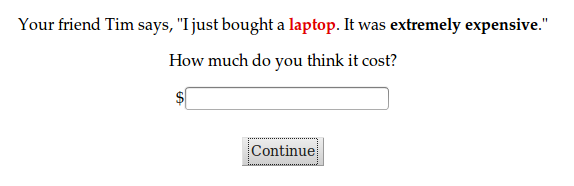
\includegraphics[width=0.4\textwidth]{analysis_files_for_writeup/images/exp1-q.png}
\end{center}
\caption{Screenshot from Experiment 1 target question.} 
\label{exp1-q}
\end{figure}

\subsubsection{Corpus Methods}
%maybe have this a separate section? maybe not?

We collected length in syllables and frequency for every intensifier (Table~\ref{exp1-intensifiers}) as measures of their cost. The frequency was collected from the Google Web 1T 5-grams database \cite{web1t5gram}\footnote{
We also ran the same analyses on frequency information collected from the Google Books American Ngrams Corpus \cite{books2011} as well, and found similar results.

In addition, we did the same using the bigram frequencies of ``\emph{[intensifer]} expensive'' rather than the unigram frequencies of the intensifiers alone. These data were much more sparse. For bigrams, we found no significant effects of surprisal using the books database and a negative effect using the web database.
}

\subsection{Results and Discussion}

If the meaning of an intensifier is stronger for higher cost intensifiers, we would expect to find that as surprisal and length in syllables increase, the prices participants give will also increase. We find that this is the case.

\begin{figure}[ht]
\begin{center}
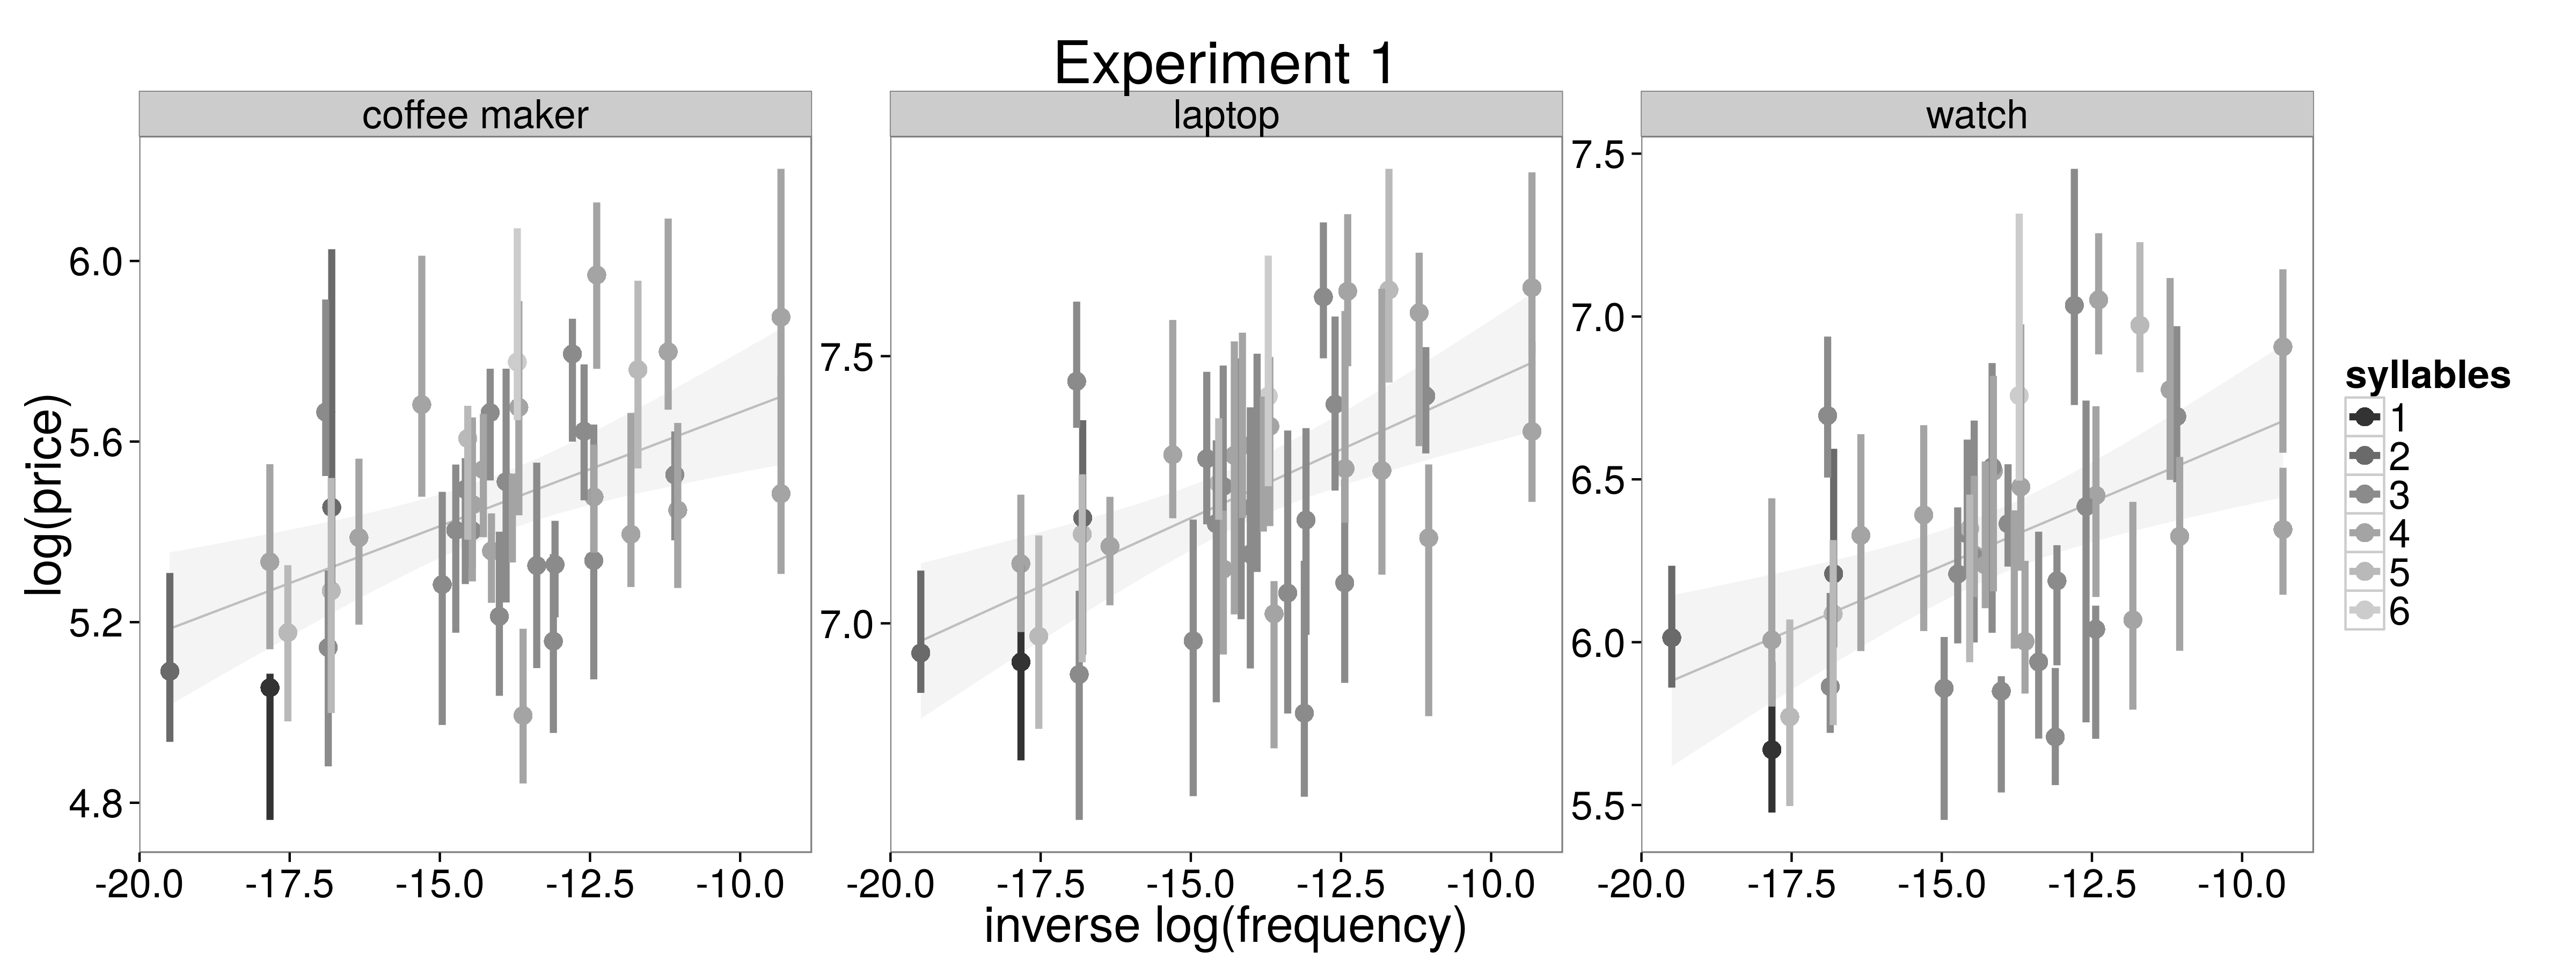
\includegraphics[width=0.48\textwidth]{analysis_files_for_writeup/images/exp1-plot.png}
\end{center}
\caption{Results of Experiment 1. As surprisal and length in syllables increase, participants' free response prices increased.} 
\label{exp1-plot}
\end{figure}

In a linear mixed effects regression with syllables and surprisal and their interaction as fixed effects\footnote{We centered both surprisal and syllable length by subtracting their means.} and random intercepts and slopes for syllables and surprisal for both participant and object, we found significant main effects of surprisal (estimate=0.054, p=0.012) and syllable length  (estimate=0.093, p=0.0041) as well as a significant interaction (estimate=0.019, p=0.00018).
%anything more complicated won't converge

This suggests that intensifiers that are more surprising and longer (and therefore are more costly to utter) also have stronger meanings.

\todo[inline]{interpret interaction}

\todo[inline]{make a big deal}

\section{Experiment 2}

In Experiment 2, we replicated our finding from Experiment 1 using a different dependent measure which we expect to be more sensitive to small differences in meaning and an extension to other adjectival scales.

\subsection{Method\footnote{The full experiment can be found at \url{http://web.stanford.edu/~erindb/degree-adverbs/experiments/exp4/exp4.html}}}

30 participants with US IP addresses participated in our Experiment 2 on Amazon's Mechanical Turk.

We divided the 40 intensifiers from Experiment 1 into four lists of 10 intensifiers each (Table~\ref{exp2-intensifiers}). Each list was randomly paired with one of four adjectives (``old'', ``expensive'', ``beautiful'', and ``tall''). For each adjective-list pairing, participants were shown every combination of the 10 intensifiers and the one adjective on the left side of the screen. They were asked to move the adjective phrases from the left to the right side of the screen, reordering the phrases from the lowest to the highest degree (Figure~\ref{exp2-q}). Each participant did four trials of this process, seeing all four lists and all four adjectives. The pairings between list and adjective were randomized between participants. The division of the intensifiers into lists of 10 was always constant, i.e. the same 10 intensifiers were always shown together.

\begin{figure}[ht]
\begin{center}
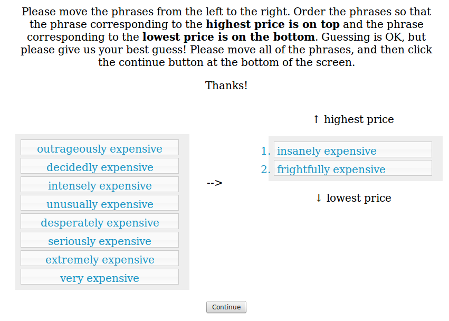
\includegraphics[width=0.4\textwidth]{analysis_files_for_writeup/images/exp2-q.png}
\end{center}
\caption{Screenshot from Experiment 2 target question.} 
\label{exp2-q}
\end{figure}

\subsection{Results and Discussion}

\todo[inline]{turns out, breaking things up by adjective, there's no significant interaction between syllables and surprisal. and there is a slight difference between the surprisal slopes for the adjectives. ``tall'' and ``expensive'' are slightly steeper than for ``beautiful'' and ``old'' (Figure~\ref{exp2-slopes}). The main effects of syllables and surprisal are  robust and almost identical across the different adjectives (Figure~\ref{exp2-main}).}

\begin{figure}[ht]
\begin{center}
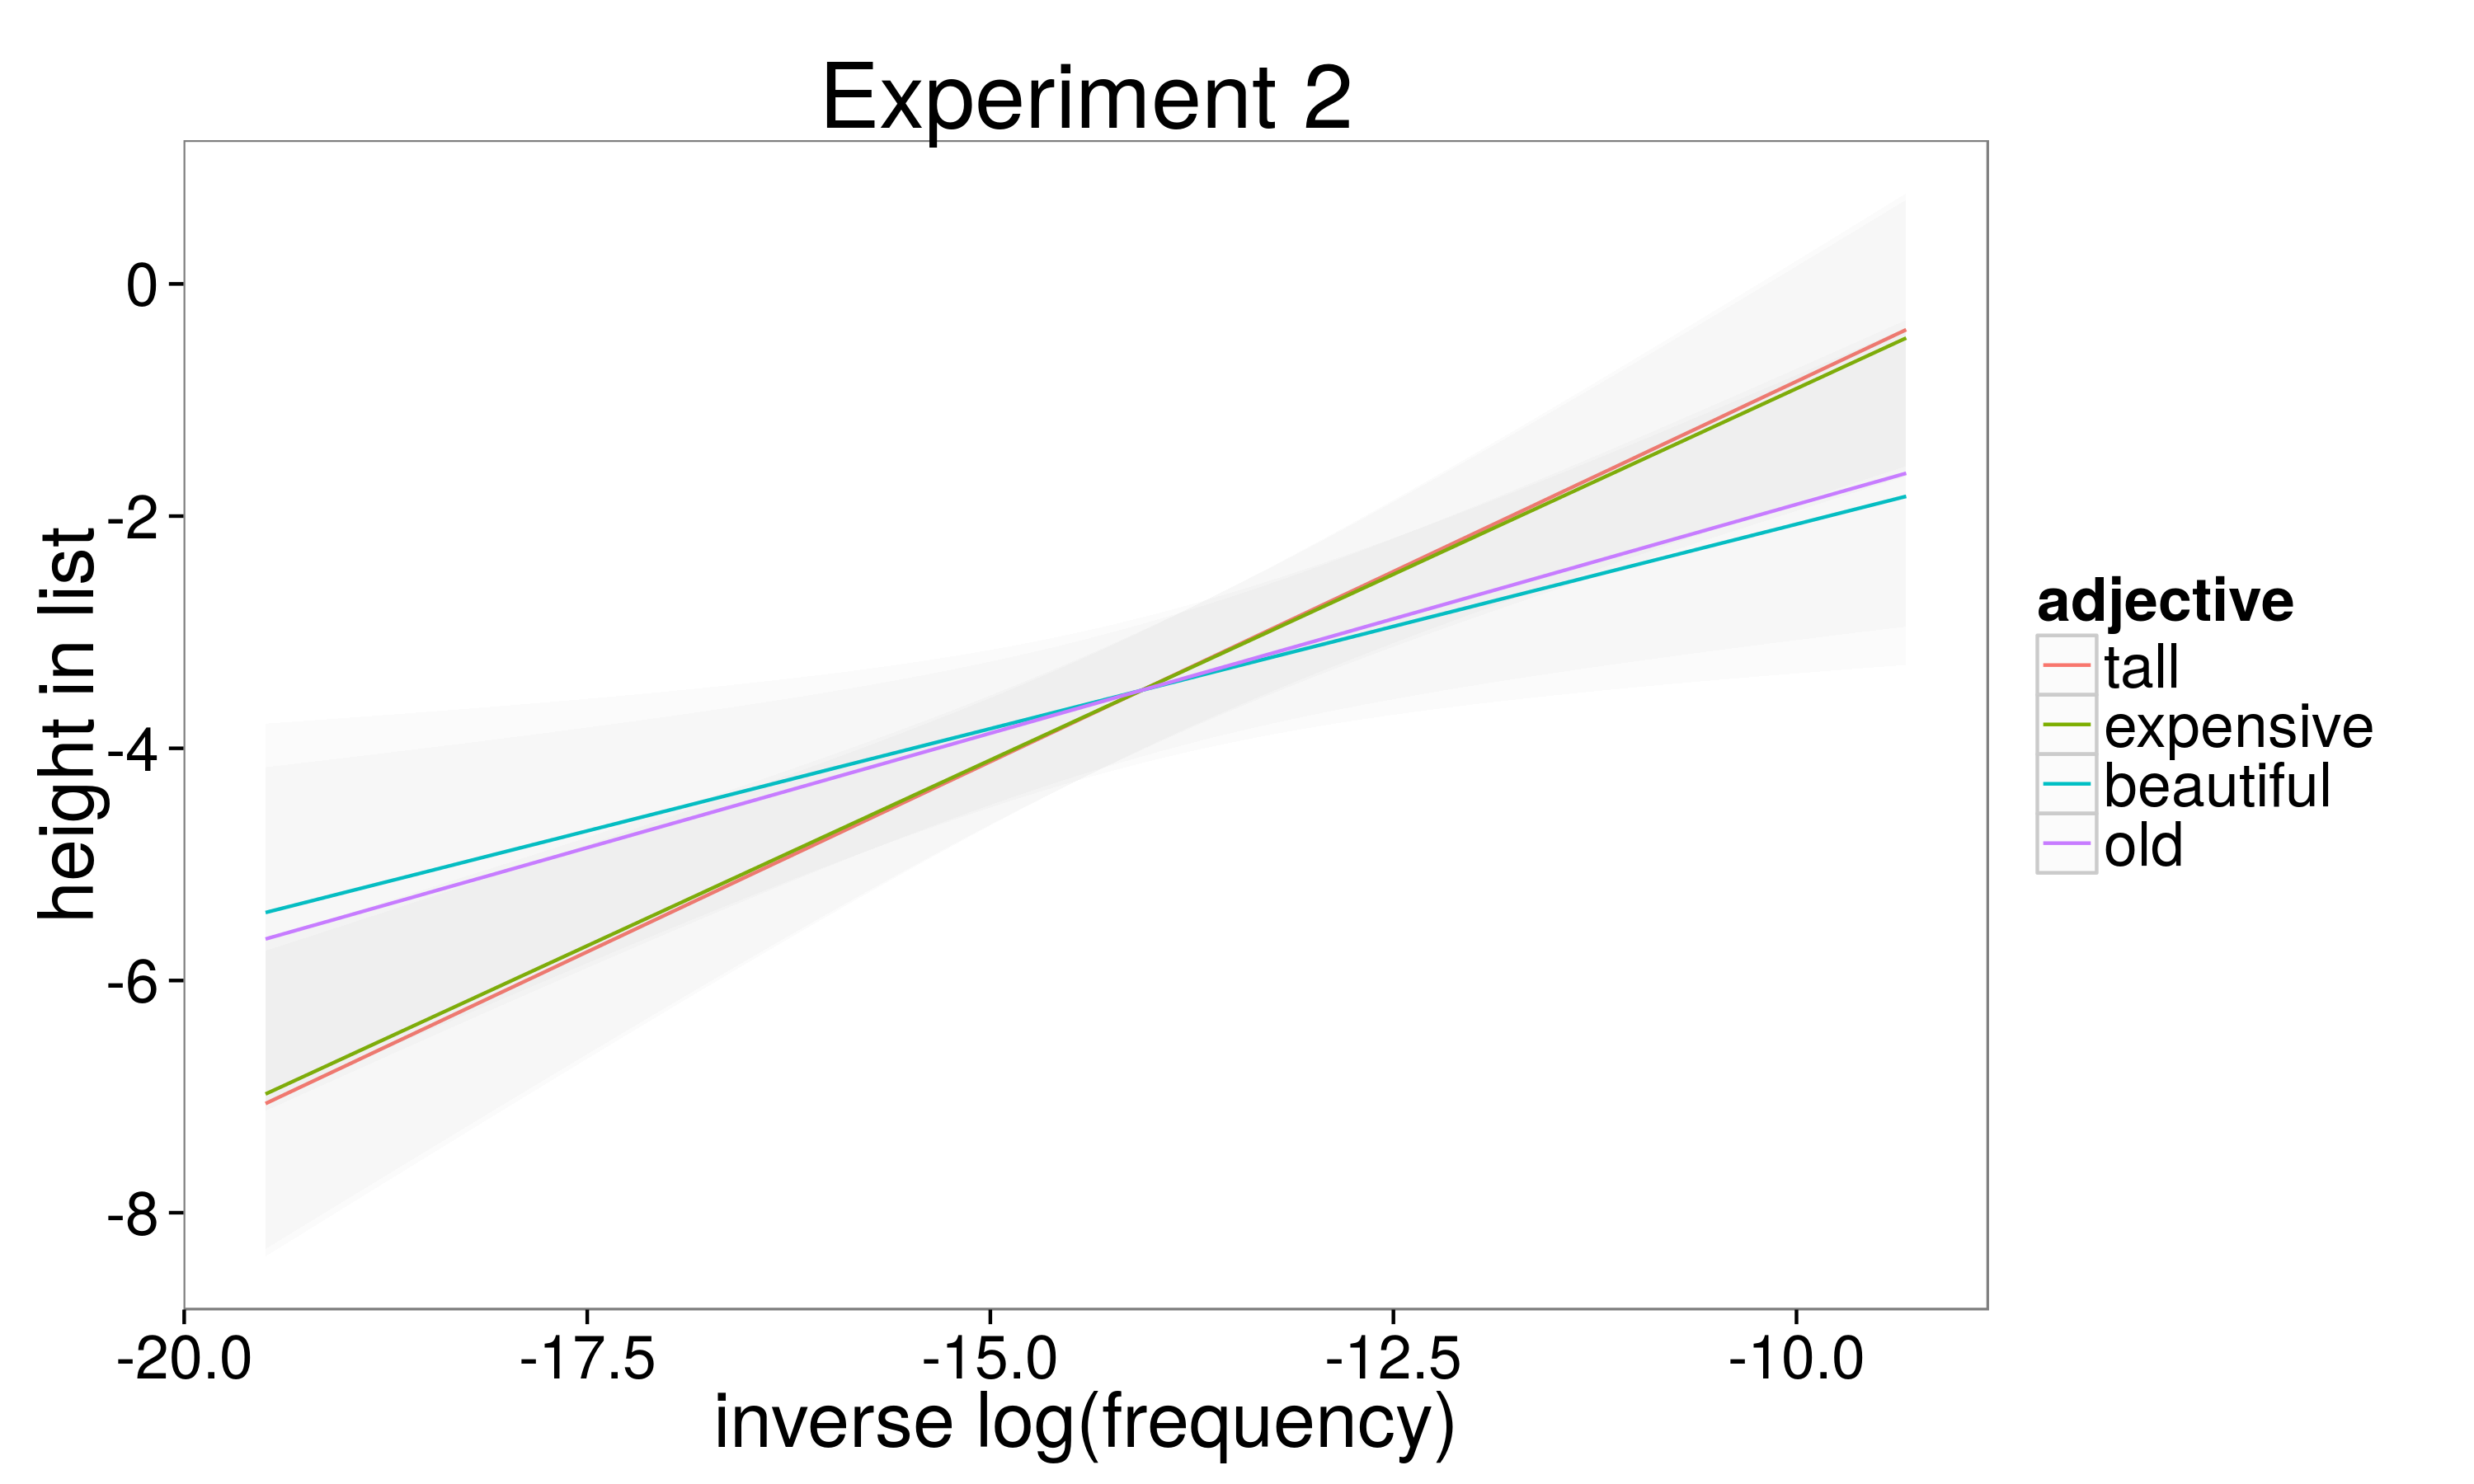
\includegraphics[width=0.48\textwidth]{analysis_files_for_writeup/images/exp2-slopes.png}
\end{center}
\caption{tall and expensive are steeper than beautiful and old} 
\label{exp2-slopes}
\end{figure}

\begin{figure}[ht]
\begin{center}
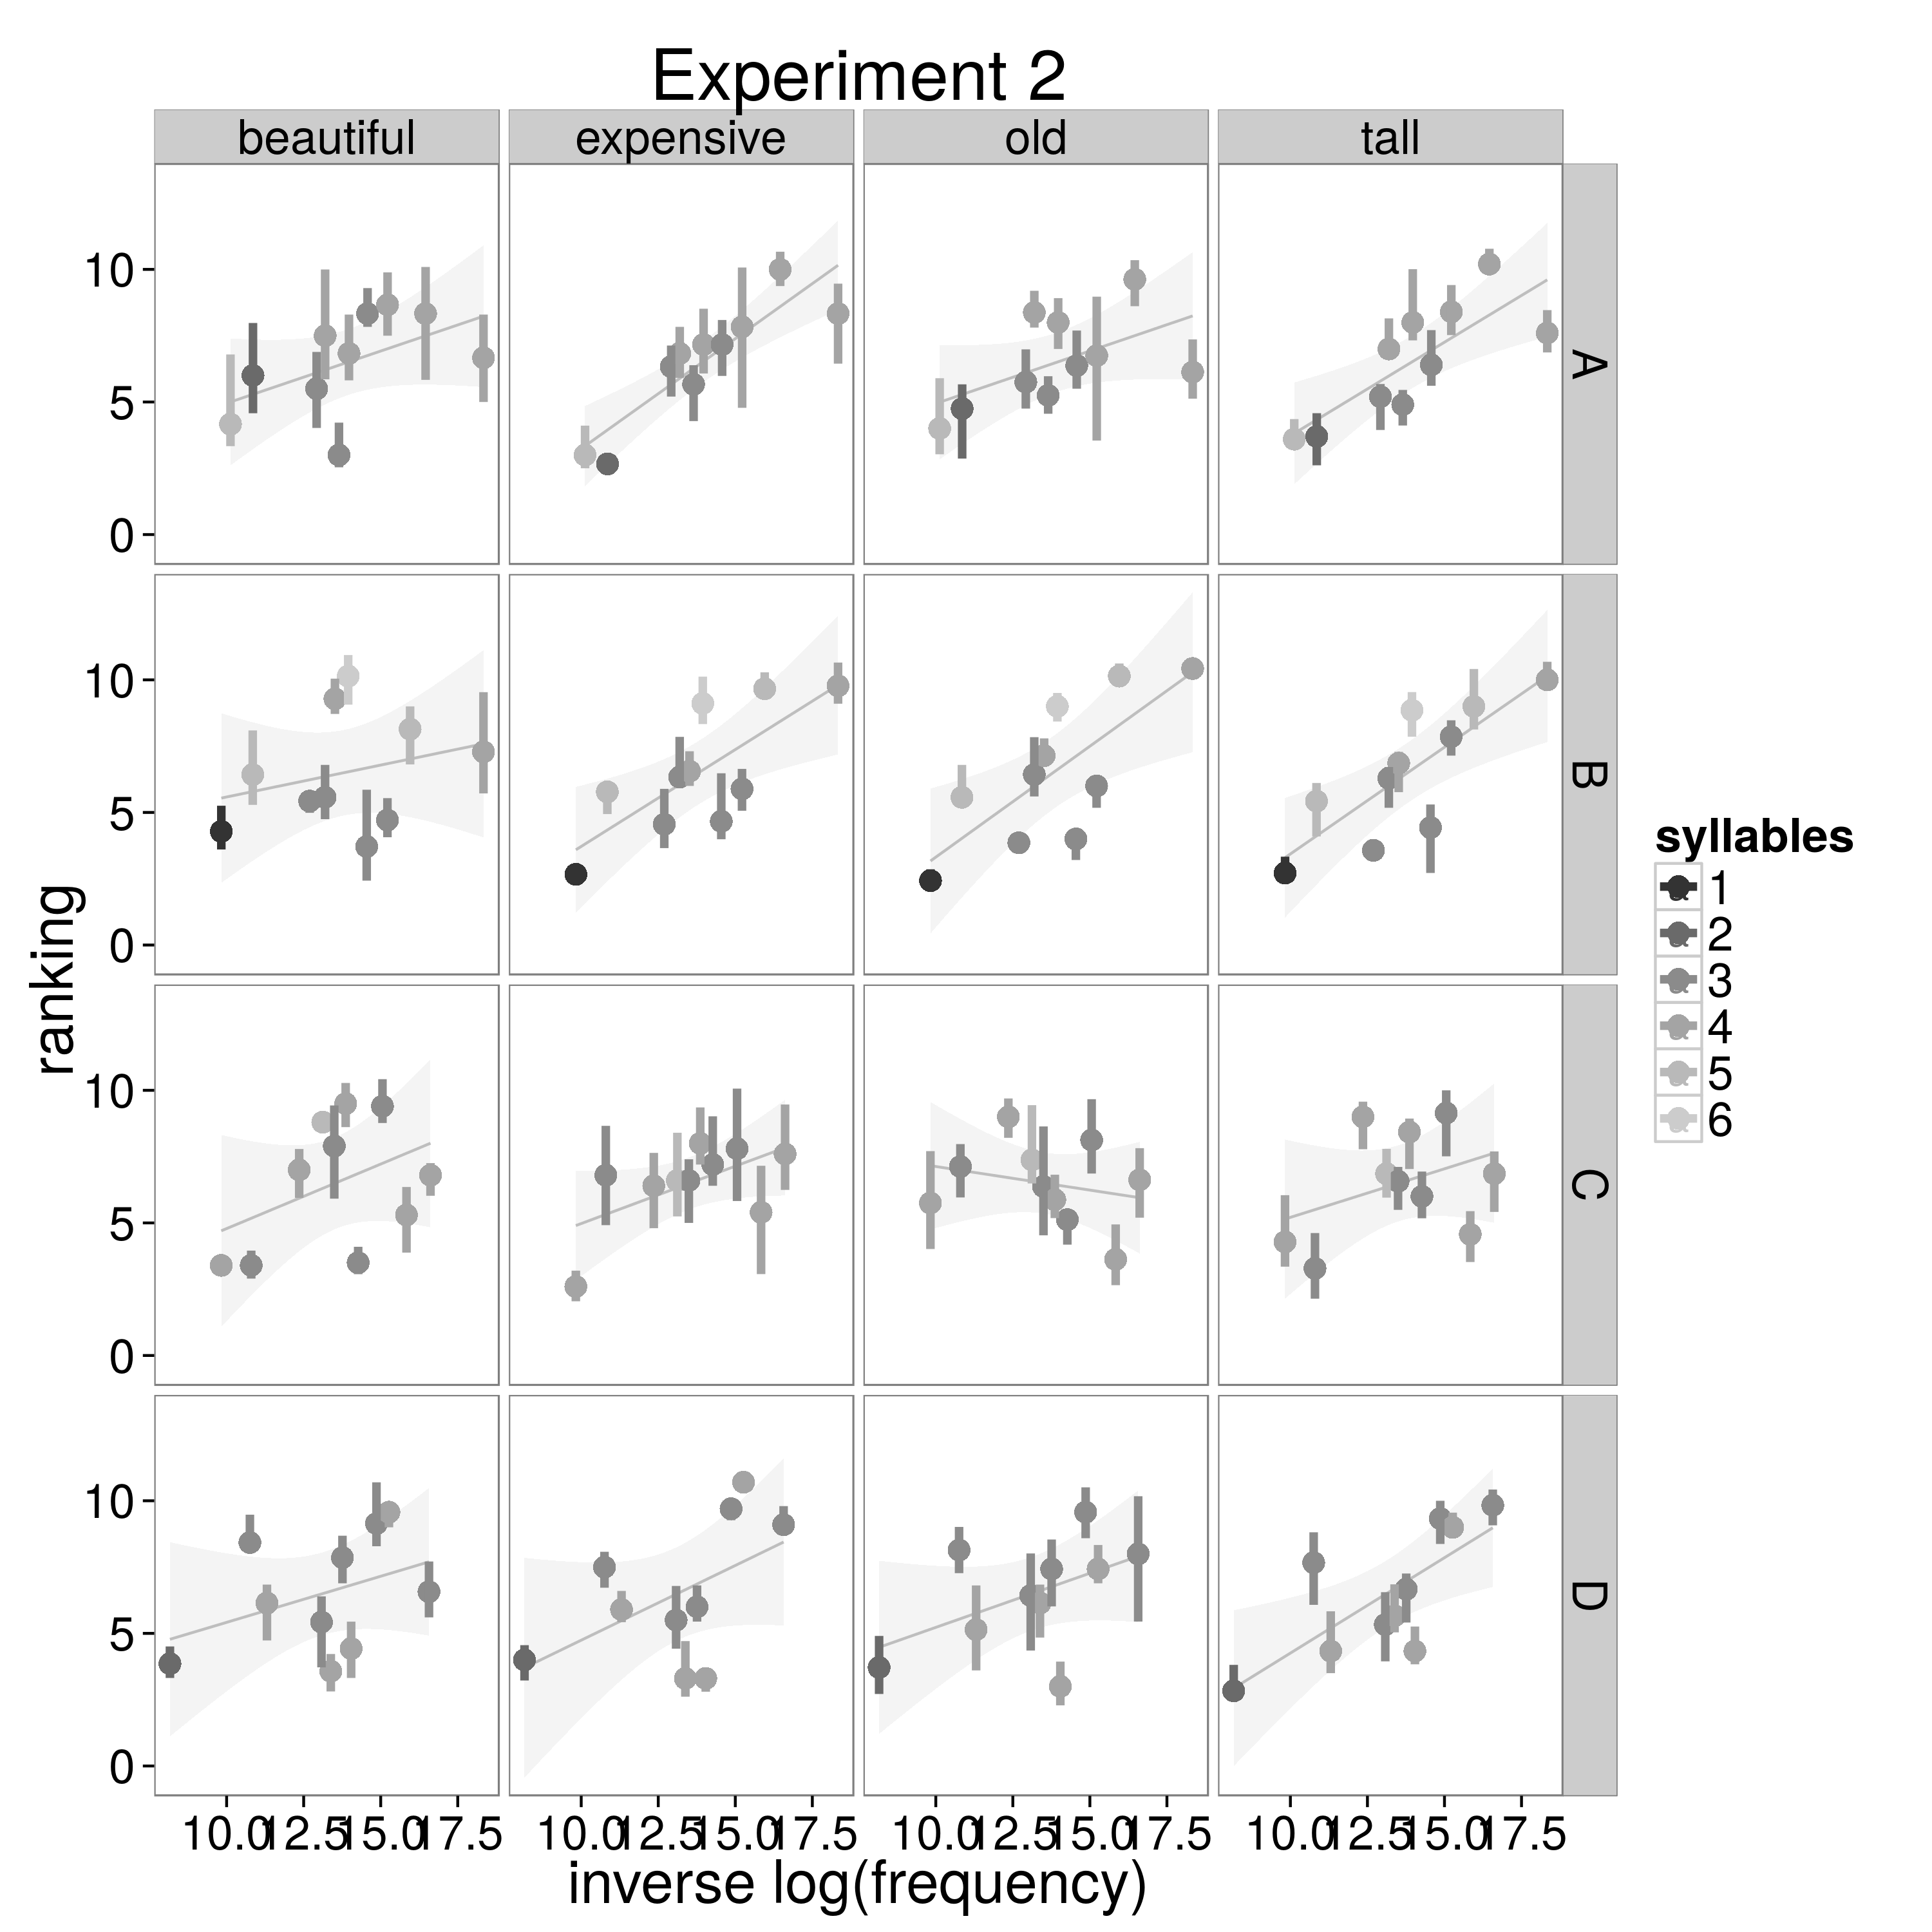
\includegraphics[width=0.48\textwidth]{analysis_files_for_writeup/images/exp2-main.png}
\end{center}
\caption{tall and expensive are steeper than beautiful and old} 
\label{exp2-main}
\end{figure}

In a linear regression of ranking within the list as a function of surprisal, syllable length, and their interaction\footnote{We centered both surprisal and syllable length by subtracting their means.}, we found significant main effects of surprisal (estimate=0.46, p$<$2e-16) and syllables (estimate=0.64, p=8.2e-11) as well as a significant interaction (estimate=0.069, p=0.046).

%expt 2 results: explain the analysis a bit more. what is being predicted? how do you combine rankings across lists? also describe the results by adj (does the result hold for each adj separately as well?). point out that this result replicates but is a much bigger effect because the measure is more sensitive.

\begin{figure}[ht]
\begin{center}

\includegraphics[width=0.48\textwidth]{analysis_files_for_writeup/images/exp2-plot.png}
\end{center}
\caption{Results of Experiment 2. As surprisal and length in syllables increase, participants' rankings increased.} 
\label{exp2-plot}
\end{figure}

We again found that participants assign stronger meanings to intensifiers with higher surprisals and syllable lengths.

The relationship between strength and suprisal could be explained by the stronger meanings themselves being more unusual and surprising and therefore corresponding to words that are used less frequently.
However, this story would not be able to explain why syllable length above and beyond surprisal would predict stronger meanings.

%before expt 3 i'd pause to interpret the results so far, bring up the question of causality (did the cost or the meaning come first?). point out that syllable effects partly address this, but then say we test it more directly by manipulating the linguistic frequency, predicting changes in meaning.

\section{Experiment 3}

In Experiment 3, we tested whether manipulating the surprisal associated with an intensifier can change the strength of an intensifier. If this were the case, it would provide more evidence for our hypothesis that the surprisal of a word causes its meaning to be stronger due to the added cost.

\subsection{Method\footnote{The full experiment can be found at \url{http://web.stanford.edu/~erindb/degree-adverbs/experiments/exp8/exp8.html}}}

\todo[inline]{i need to clean this up}
%expt 3: describe the training story a bit more: length, content, etc.

We looked at two short intensifiers of equal length: ``truly'' and ``very''. In our two conditions (varied between participants), each intensifier was either the target or the control. In a comic-style training story, the target intensifier was repeated 22 times by a speaker who lived ``across the country'' and had ``a distinct way of speaking.'' The control intensifier was not used by the speaker in the story.

To guage whether participants had learned that the speaker's use of the target intensifier was unusually high, we asked participants how many times in the next 1000 words they thought the speaker would use the control word, the target word, and another word that had been frequently repeated.

To determine what strength participants inferred for the target and control intensifiers, we gave participants a final panel of the comic where the speaker described a new coffee maker he bought (Fig~\ref{exp3-q}). We asked participants to guess the price of the coffee maker given different possible descriptions the speaker could have used.

\begin{figure}[ht]
\begin{center}
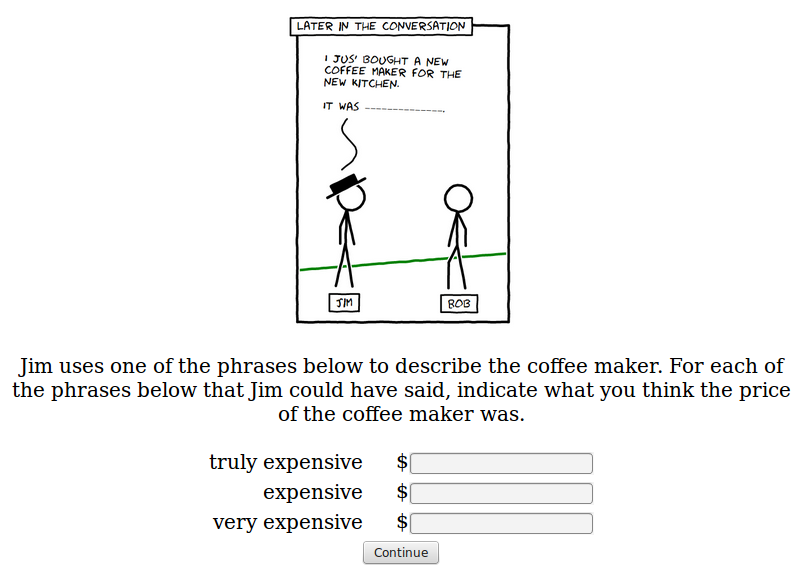
\includegraphics[width=0.4\textwidth]{analysis_files_for_writeup/images/exp3-q.png}
\end{center}
\caption{Screenshot from Experiment 3 target question.} 
\label{exp3-q}
\end{figure}

\subsection{Results and Discussion}

\todo[inline]{i need to clean this up}

%take another pass cleaning up the presentation of expt 3 results. ;)

We found that participants did learn that the speaker's use of a word was much higher when it was a target than when it was a control (Fig~\ref{exp3-freq-plot}). In a linear regression with word type (target or control) as a fixed effect and random intercepts for word and participant, word type was a significant predictor of frequency (estimate=34.06, p=0.0405).

In addition, when participants believed the speaker's use of a word was much higher, they believed the meaning the speaker intended to convey with the word was lower (Fig~\ref{exp3-price-plot}). The difference between ``\emph{(truly$|$very)} expensive'' and ``expensive'' was greater for the target word than for the control word. In a linear gregression with word type as a fixed effect and random intercepts for word and participant, word type was a significant predictor of difference score (estimate=-31.39, p=0.0226).

In a linear regression with word type (target or control) as a fixed effect and random intercepts for word and participant, word type was a significant predictor of frequency (estimate=34.06, p=0.0405).

Individuals' estimates of frequency correlate with their estimates of price (Fig~\ref{exp3-scatterplot}, Pearson's r=0.396, p=0.0169).

\begin{figure}[ht]
\begin{center}
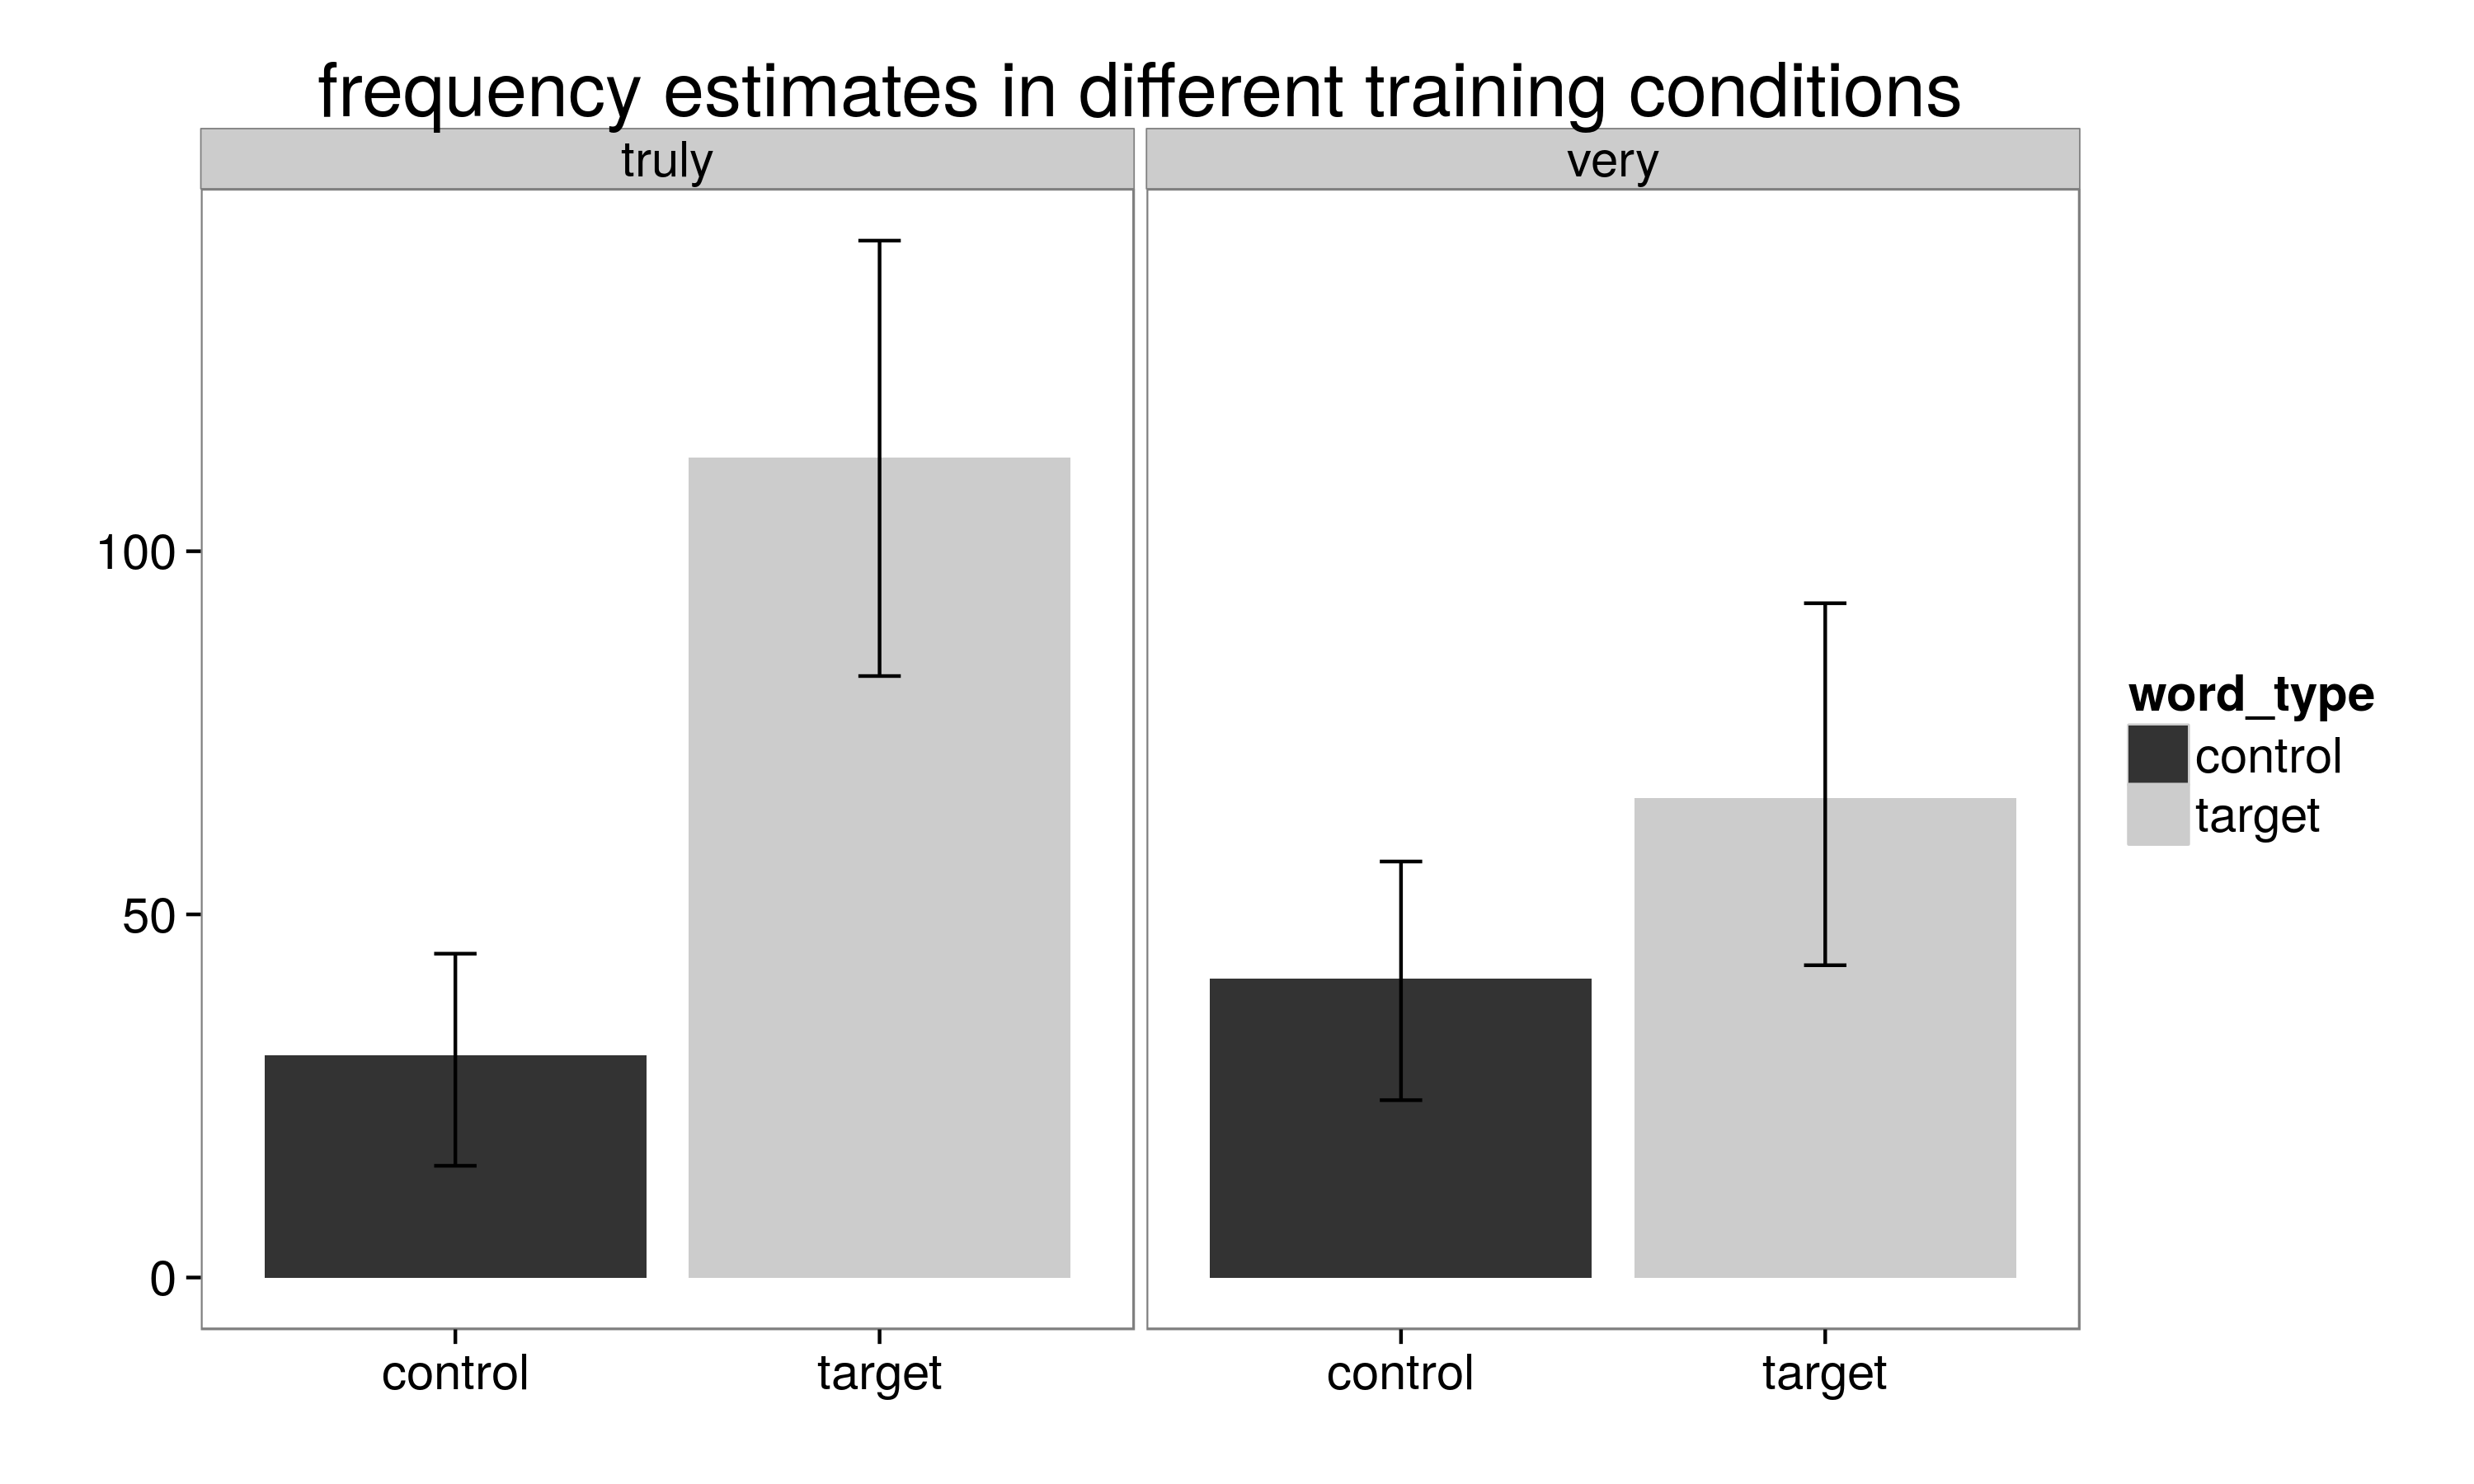
\includegraphics[width=0.48\textwidth]{analysis_files_for_writeup/images/exp3-freq-plot}
\end{center}
\caption{Results of Experiment 3. Intensifier is given a higher frequency estimate when it is target than when it is control, showing that participants learned a new frequency for that intensifier from the training.} 
\label{exp3-freq-plot}
\end{figure}

\begin{figure}[ht]
\begin{center}
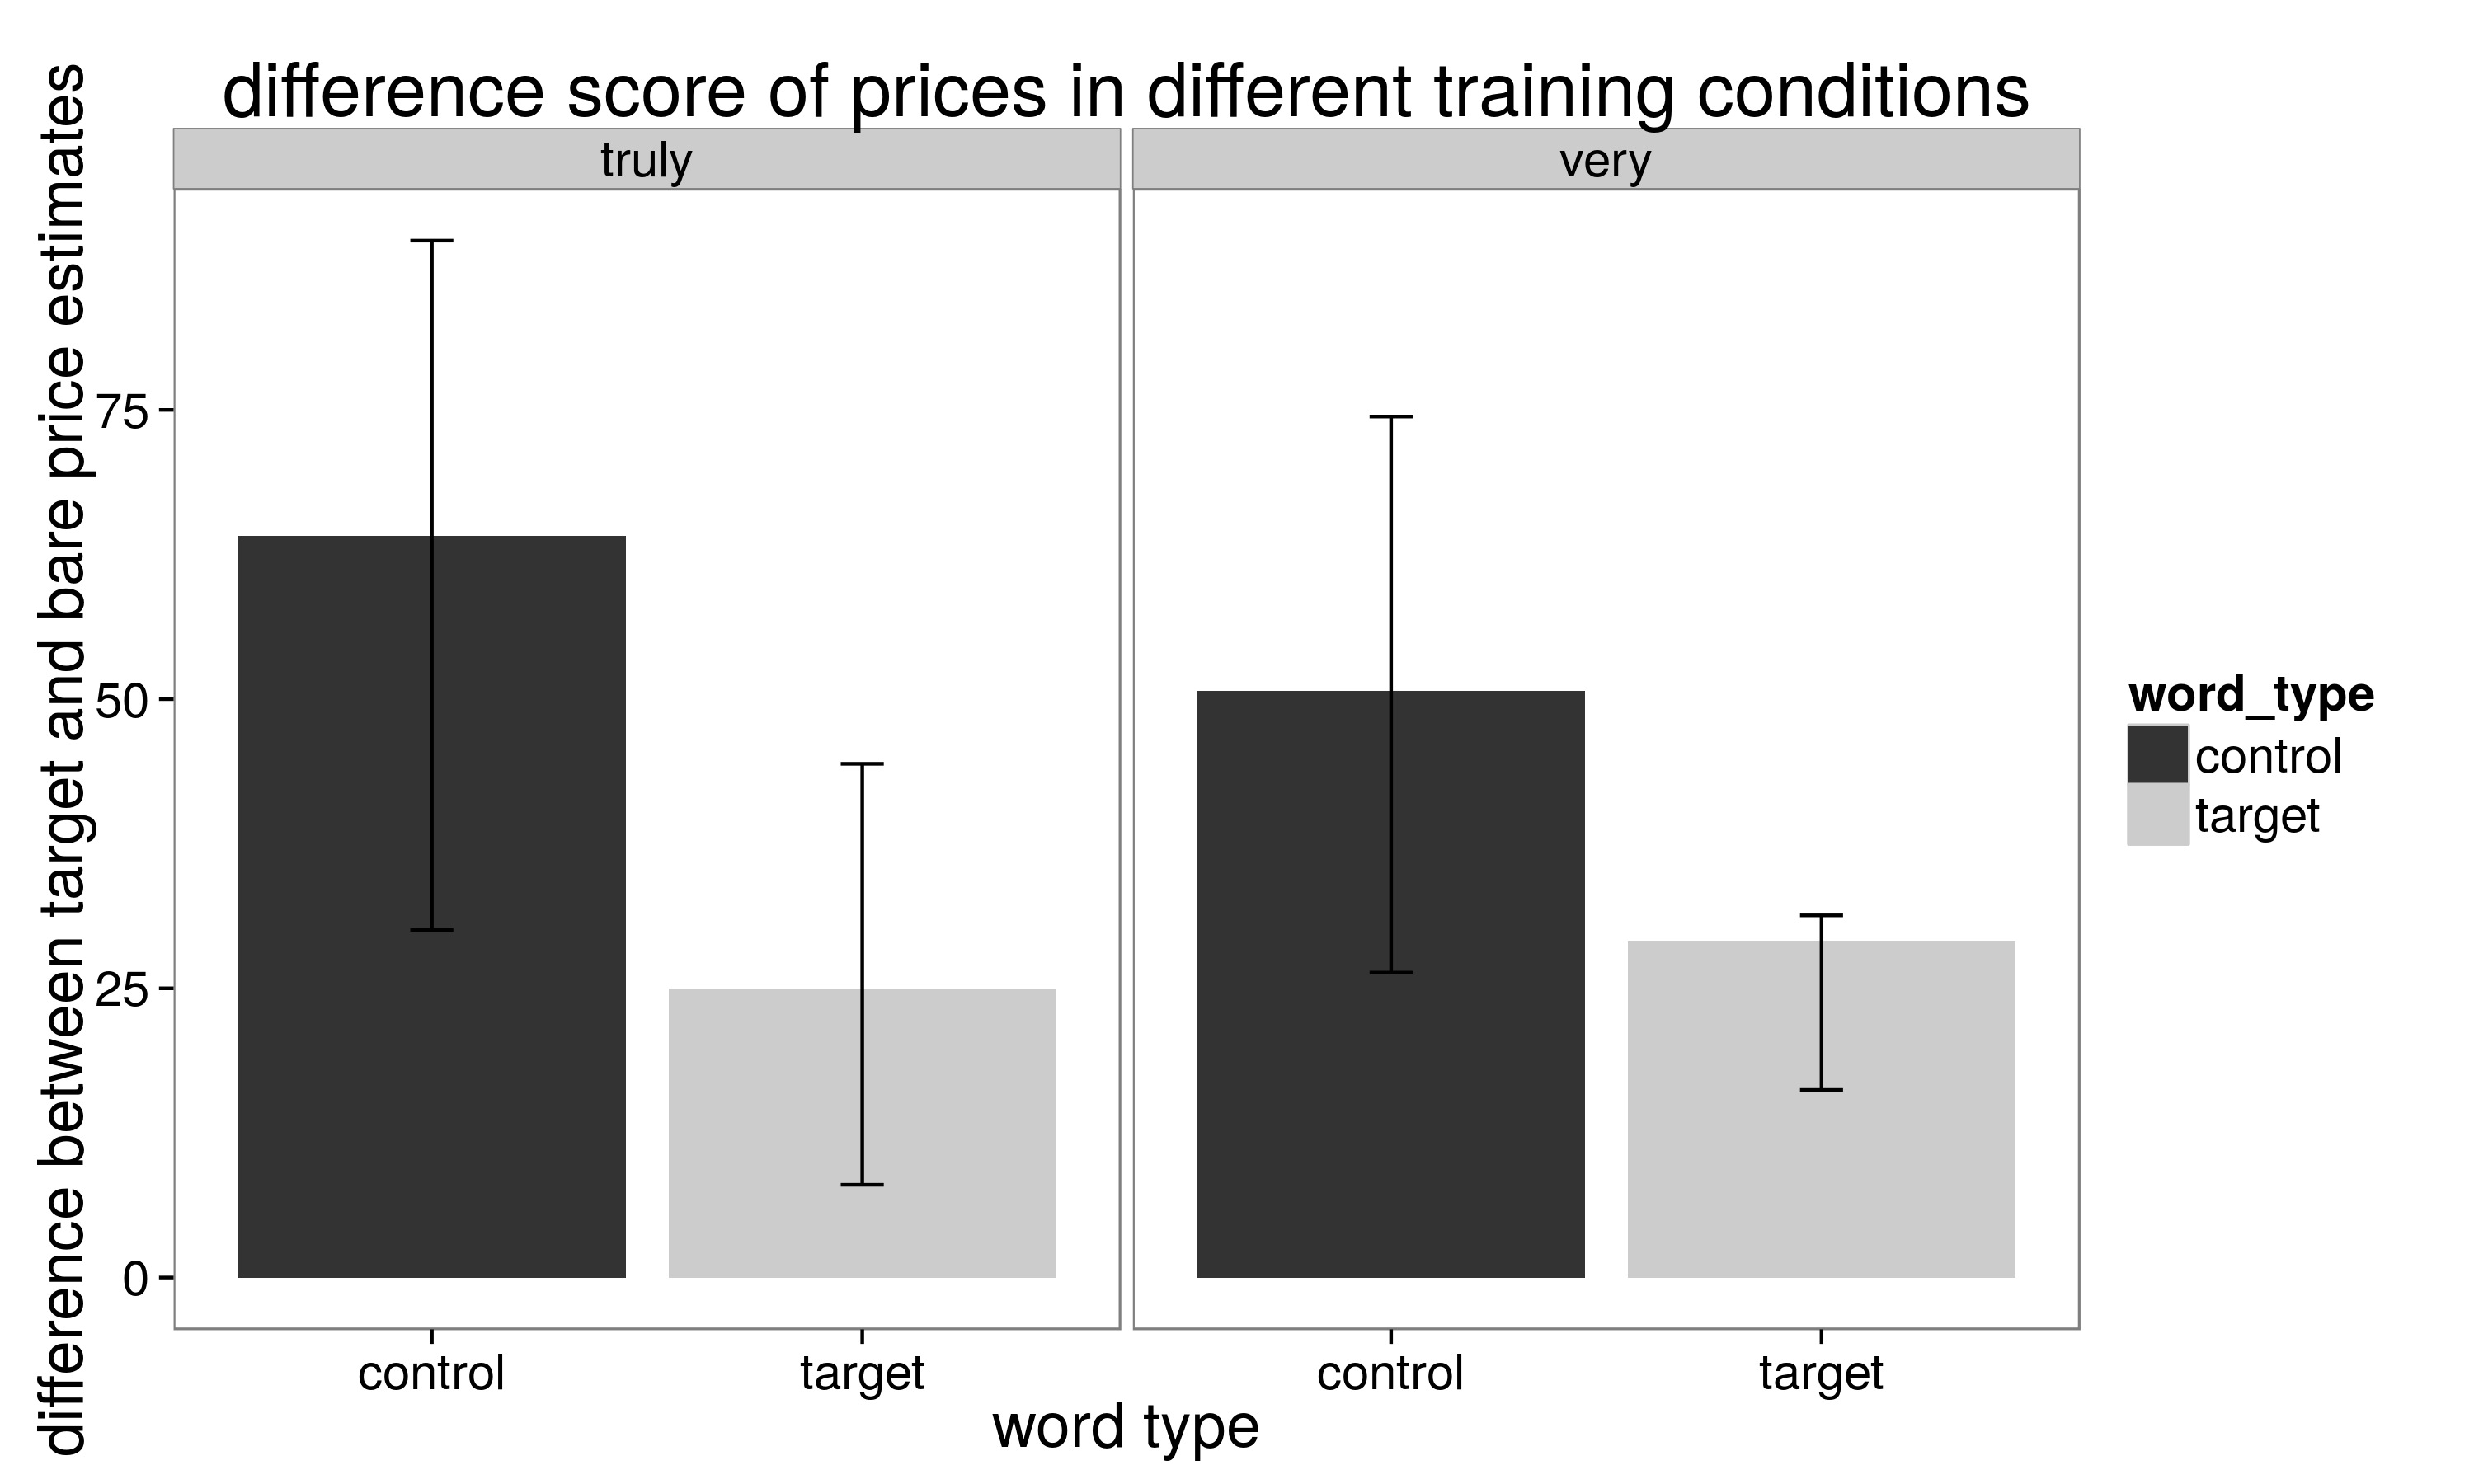
\includegraphics[width=0.48\textwidth]{analysis_files_for_writeup/images/exp3-price-plot.png}
\end{center}
\caption{Results of Experiment 3. Price estimate for intensifier is lower after the intensifier is repeated (target condition), showing that overuse within a dialect results in a less strong meaning.} 
\label{exp3-price-plot}
\end{figure}

\begin{figure}[ht]
\begin{center}
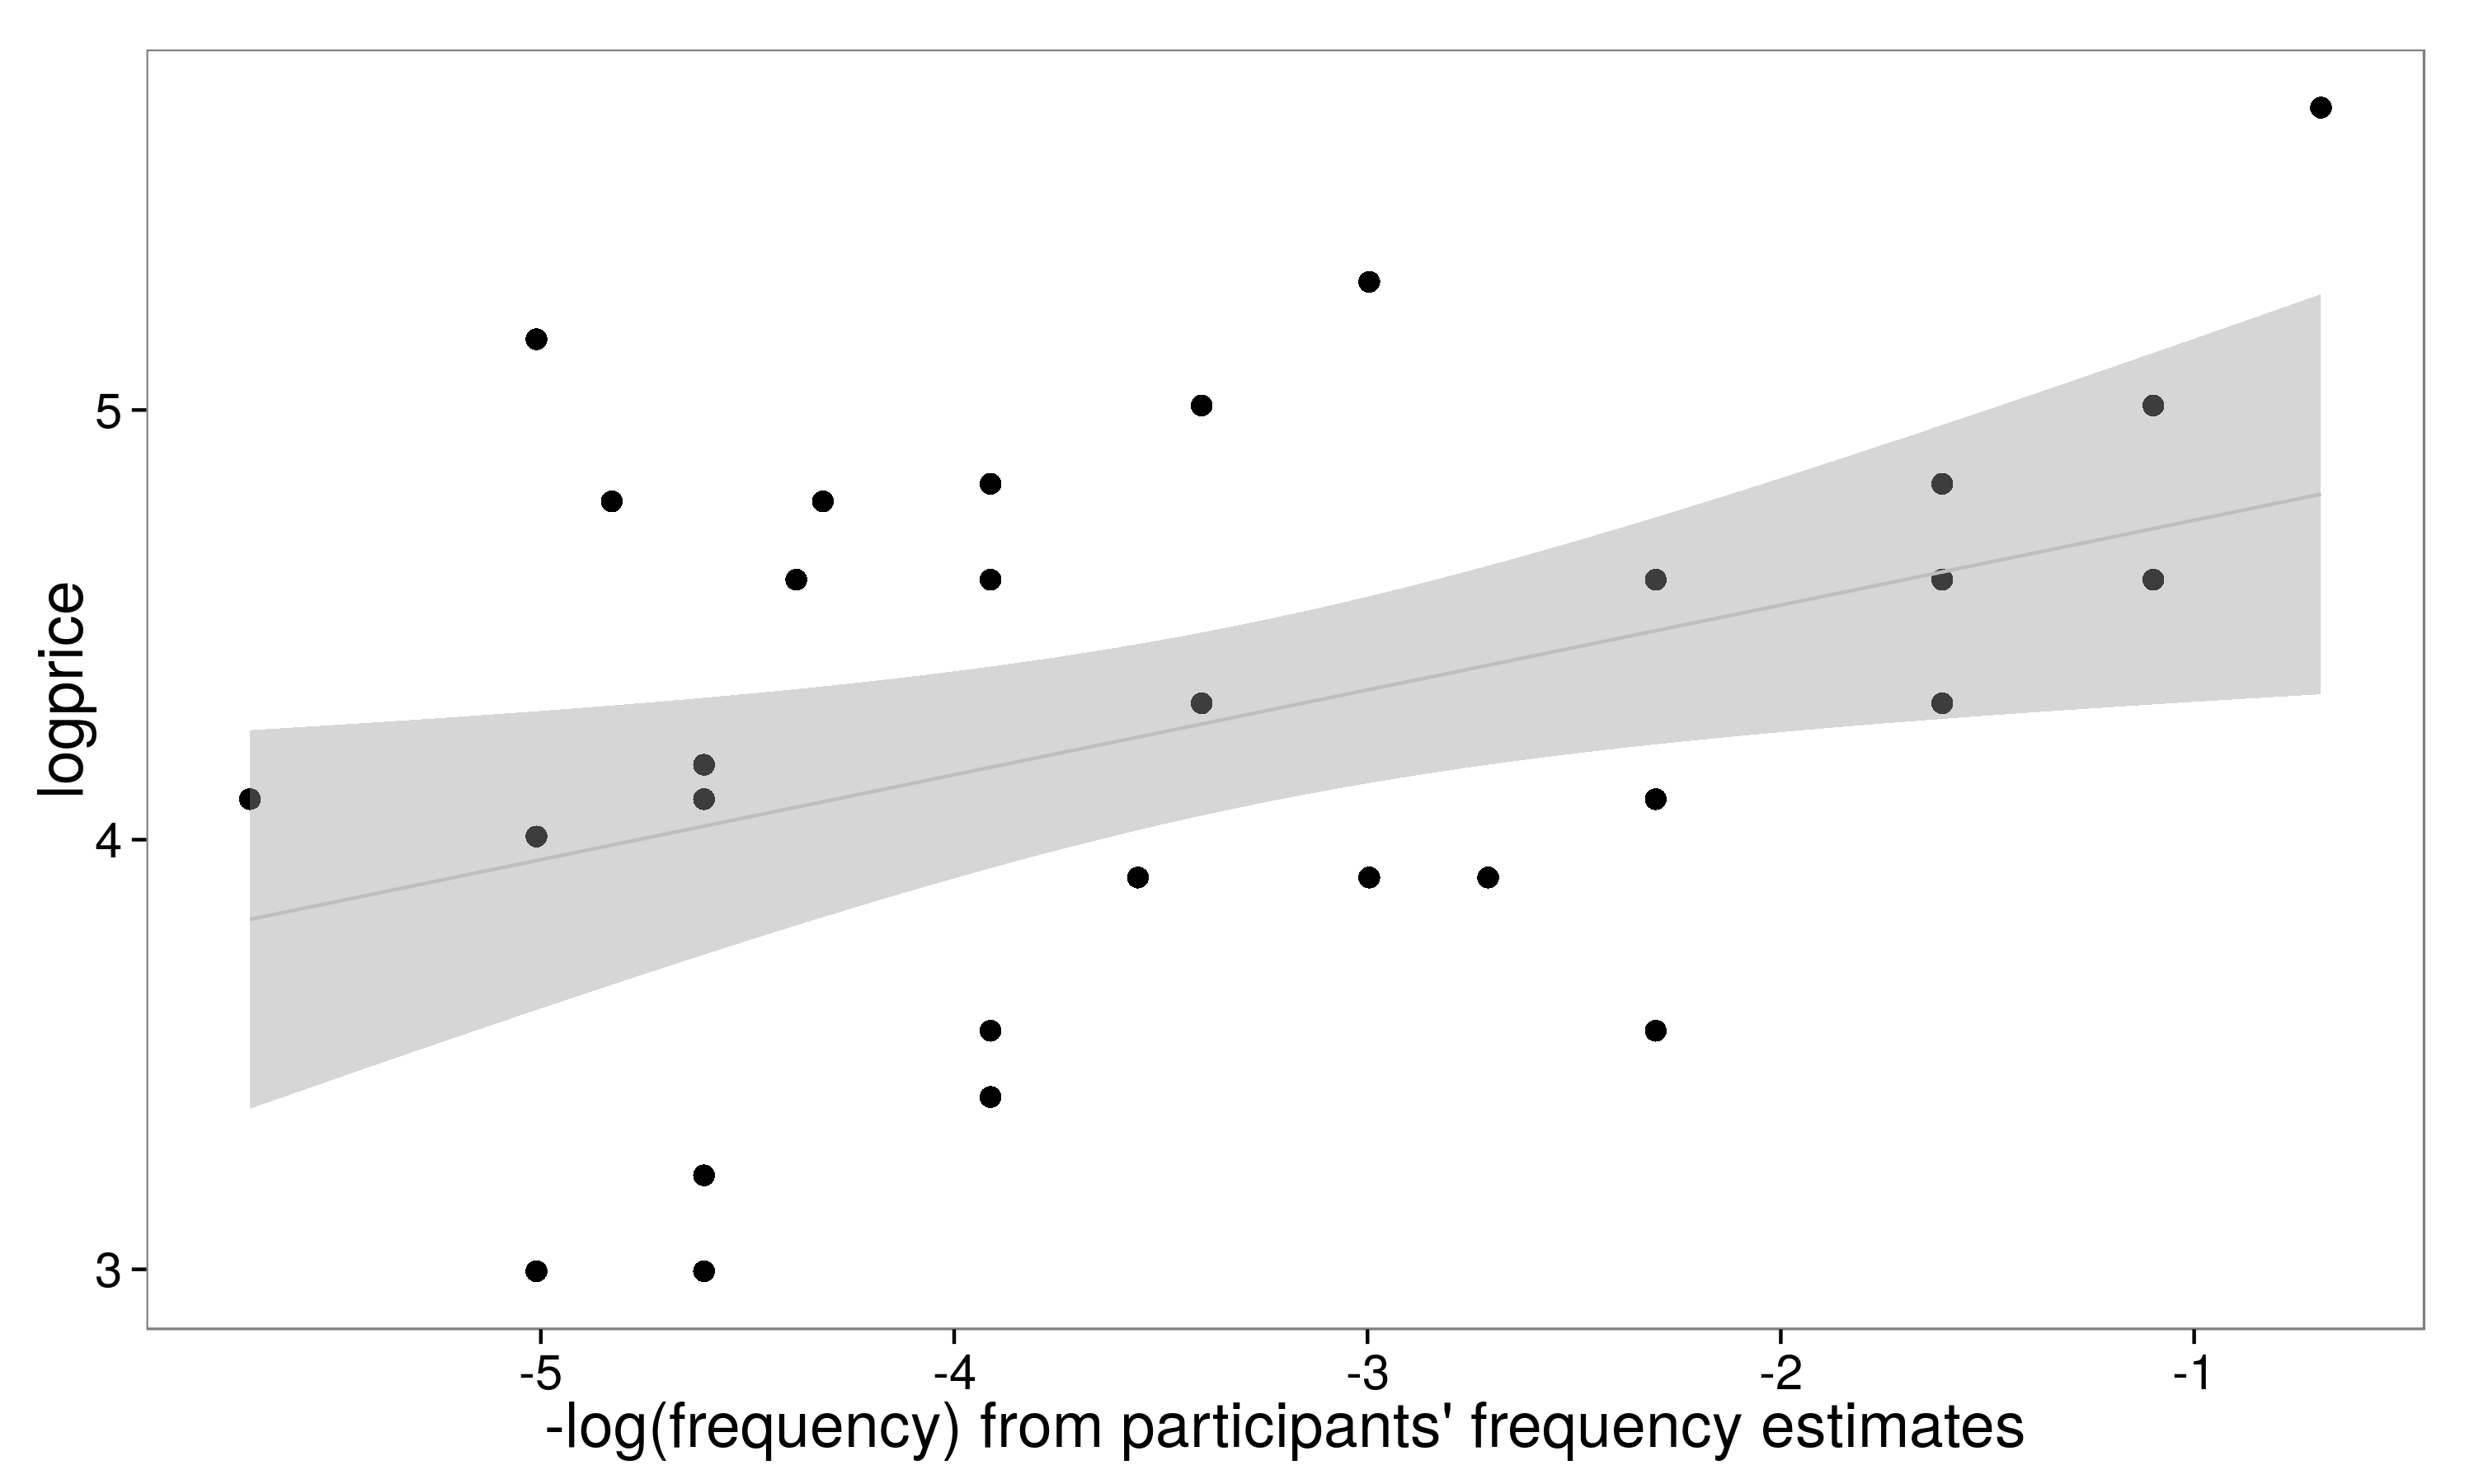
\includegraphics[width=0.48\textwidth]{analysis_files_for_writeup/images/exp3-scatterplot.png}
\end{center}
\caption{Results of Experiment 3. As participants' frequency estimates increase, their price estimates decrease.} 
\label{exp3-scatterplot}
\end{figure}

%do we have any way of estimating how much of an intensifier's meaning is determined by freq and syll? i'm not exactly sure how we would do this... maybe something like residual information not accounted for?

\section{Discussion}

%in general discussion / conclusion should address again the thing from the intro, also talk about other aspects of meaning (eg affect), issues with our results, and some future directions.

\todo[inline]{conclusion}

\section{Acknowledgments}

\nocite{web1t5gram}
\nocite{lewis}

\begin{table}[ht]
 \begin{center}
  \caption{Intensifiers from Experiment 1, number of occurences in Google Web 1T 5grams corpus, and number of syllables.}
  \label{exp1-intensifiers}
  \begin{tabular}{ccc}
   \hline
   ngram & frequency & syllables \\
    \hline
    surpassingly & 11156 & 4 \\
    colossally & 11167 & 4 \\
    terrifically & 62292 & 4 \\
    frightfully & 65389 & 3 \\
    astoundingly & 73041 & 4 \\
    phenomenally & 120769 & 5 \\
    uncommonly & 135747 & 4 \\
    outrageously & 240010 & 4 \\
    fantastically & 250989 & 4 \\
    mightily & 252135 & 3 \\
    supremely & 296134 & 3 \\
    insanely & 359644 & 3 \\
    strikingly & 480417 & 3 \\
    acutely & 493931 & 3 \\
    awfully & 651519 & 3 \\
    decidedly & 817806 & 4 \\
    excessively & 877280 & 4 \\
    extraordinarily & 900456 & 6 \\
    exceedingly & 977435 & 4 \\
    intensely & 1084765 & 3 \\
    markedly & 1213704 & 3 \\
    amazingly & 1384225 & 4 \\
    radically & 1414254 & 3 \\
    unusually & 1583939 & 4 \\
    remarkably & 1902493 & 4 \\
    terribly & 1906059 & 3 \\
    exceptionally & 2054231 & 5 \\
    desperately & 2139968 & 3 \\
    utterly & 2507480 & 3 \\
    notably & 3141835 & 3 \\
    incredibly & 4416030 & 4 \\
    seriously & 12570333 & 4 \\
    truly & 19778608 & 2 \\
    significantly & 19939125 & 5 \\
    totally & 20950052 & 3 \\
    extremely & 21862963 & 3 \\
    particularly & 41066217 & 5 \\
    quite & 55269390 & 1 \\
    especially & 55397873 & 4 \\
    very & 292897993 & 2
  \end{tabular}
 \end{center}
\end{table}


\begin{table}[ht]
\begin{center} 
\caption{Intensifier Lists from Experiment 2: Rankings.} 
\label{exp2-intensifiers} 
\vskip 0.12in
\begin{tabular}{cccc} 
\hline
List A    &  List B & List C & List D \\
\hline
surpassingly & colossally & terrifically & frightfully \\
astoundingly & phenomenally & uncommonly & outrageously \\
fantastically & mightily & supremely & insanely \\
strikingly & acutely & awfully & decidedly \\
excessively & extraordinarily & exceedingly & intensely \\
markedly & amazingly & radically & unusually \\
remarkably & terribly & exceptionally & desperately \\
utterly & notably & incredibly & seriously \\
truly & significantly & totally & extremely \\
particularly & quite & especially & very
\end{tabular}
\end{center}
\end{table}


\begin{figure}
        \centering
        \begin{subfigure}[b]{0.45\textwidth}
                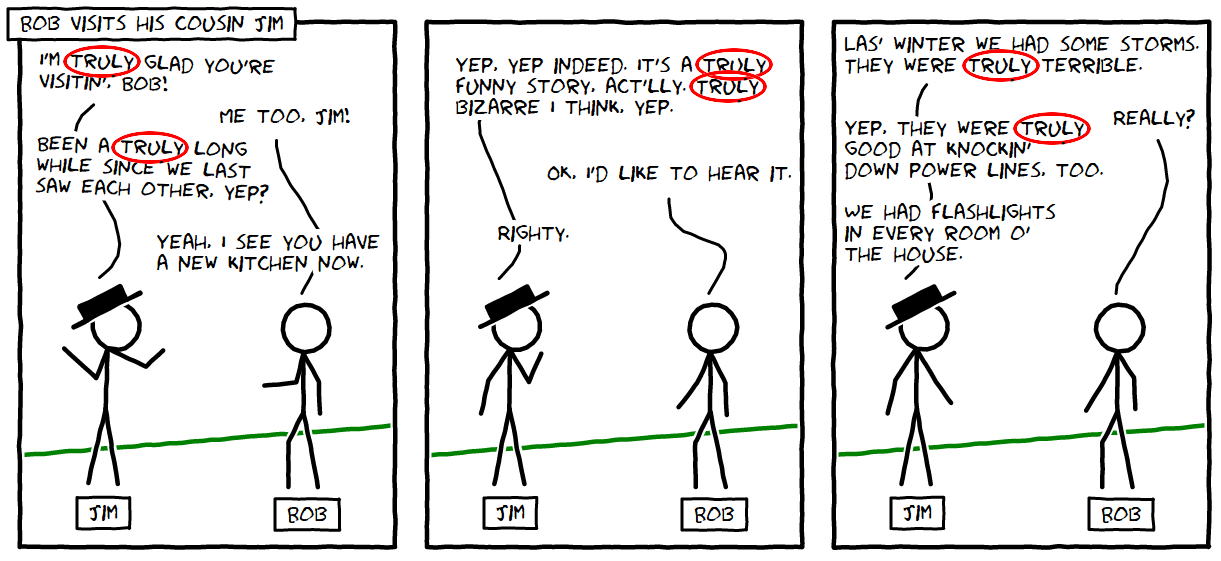
\includegraphics[width=\textwidth]{analysis_files_for_writeup/images/story1_truly_circles.png}
        \end{subfigure}%
        
        \begin{subfigure}[b]{0.45\textwidth}
                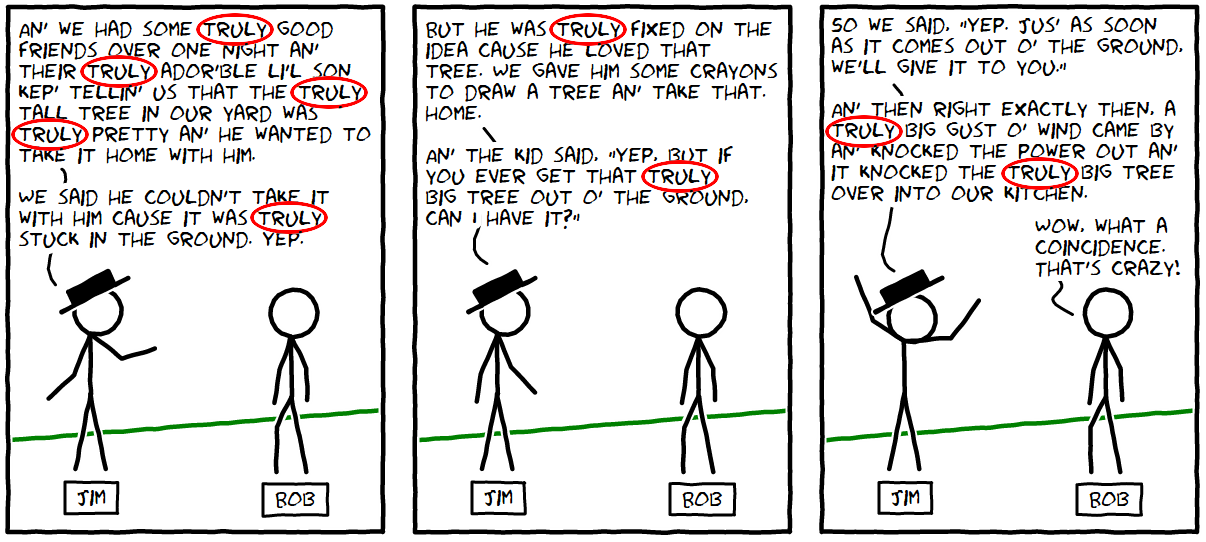
\includegraphics[width=\textwidth]{analysis_files_for_writeup/images/story2_truly_circles.png}
        \end{subfigure}
        
        \begin{subfigure}[b]{0.45\textwidth}
                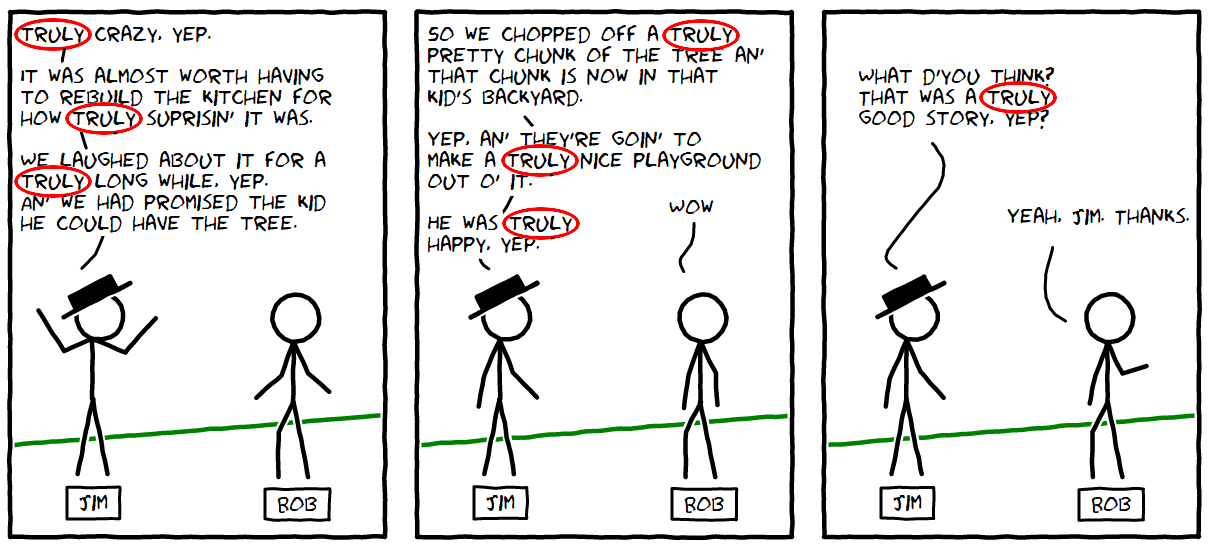
\includegraphics[width=\textwidth]{analysis_files_for_writeup/images/story3_truly_circles.png}
        \end{subfigure}
        \caption{Full comic for Experiment 3, target intensifier ``truly'' is repeated 22 times, control target ``very'' is not used.}\label{exp3-story}
\end{figure}


\bibliographystyle{apacite}

\setlength{\bibleftmargin}{.125in}
\setlength{\bibindent}{-\bibleftmargin}

\bibliography{intensifiers}

\end{document}
